\documentclass[12pt]{article}

\usepackage{amsmath, mathtools}
\usepackage{amsfonts}
\usepackage{amssymb}
\usepackage{graphicx}
\usepackage{colortbl}
\usepackage{xr}
\usepackage{hyperref}
\usepackage{longtable}
\usepackage{xfrac}
\usepackage{tabularx}
\usepackage{float}
\usepackage{siunitx}
\usepackage{booktabs}
\usepackage{caption}
\usepackage{pdflscape}
\usepackage{afterpage}

\usepackage[round]{natbib}
%\usepackage{refcheck}

\hypersetup{
    bookmarks=true,         % show bookmarks bar?
    colorlinks=true,       % false: boxed links; true: colored links
    linkcolor=red,          % color of internal links (change box color with linkbordercolor)
    citecolor=green,        % color of links to bibliography
    filecolor=magenta,      % color of file links
    urlcolor=cyan           % color of external links
}

%% Comments

\usepackage{color}

%\newif\ifcomments\commentstrue %displays comments
\newif\ifcomments\commentsfalse %so that comments do not display

\ifcomments
\newcommand{\authornote}[3]{\textcolor{#1}{[#3 ---#2]}}
\newcommand{\todo}[1]{\textcolor{red}{[TODO: #1]}}
\else
\newcommand{\authornote}[3]{}
\newcommand{\todo}[1]{}
\fi

\newcommand{\wss}[1]{\authornote{blue}{SS}{#1}} 
\newcommand{\plt}[1]{\authornote{magenta}{TPLT}{#1}} %For explanation of the template
\newcommand{\an}[1]{\authornote{cyan}{Author}{#1}}

%% Common Parts

\newcommand{\progname}{Mechatronics Engineering} % PUT YOUR PROGRAM NAME HERE
\newcommand{\authname}{Team 25, Preliminary
\\ Ahmed Nazir, nazira1
\\ Stephen Oh, ohs9
\\ Muhanad Sada, sadam
\\ Tioluwalayomi Babayeju, babayejt} % AUTHOR NAMES                  

\usepackage{hyperref}
    \hypersetup{colorlinks=true, linkcolor=blue, citecolor=blue, filecolor=blue,
                urlcolor=blue, unicode=false}
    \urlstyle{same}
                                


% For easy change of table widths
\newcommand{\colZwidth}{1.0\textwidth}
\newcommand{\colAwidth}{0.13\textwidth}
\newcommand{\colBwidth}{0.82\textwidth}
\newcommand{\colCwidth}{0.1\textwidth}
\newcommand{\colDwidth}{0.05\textwidth}
\newcommand{\colEwidth}{0.8\textwidth}
\newcommand{\colFwidth}{0.17\textwidth}
\newcommand{\colGwidth}{0.5\textwidth}
\newcommand{\colHwidth}{0.28\textwidth}

% Used so that cross-references have a meaningful prefix
\newcounter{defnum} %Definition Number
\newcommand{\dthedefnum}{GD\thedefnum}
\newcommand{\dref}[1]{GD\ref{#1}}
\newcounter{datadefnum} %Datadefinition Number
\newcommand{\ddthedatadefnum}{DD\thedatadefnum}
\newcommand{\ddref}[1]{DD\ref{#1}}
\newcounter{theorynum} %Theory Number
\newcommand{\tthetheorynum}{T\thetheorynum}
\newcommand{\tref}[1]{T\ref{#1}}
\newcounter{tablenum} %Table Number
\newcommand{\tbthetablenum}{T\thetablenum}
\newcommand{\tbref}[1]{TB\ref{#1}}
\newcounter{assumpnum} %Assumption Number
\newcommand{\atheassumpnum}{P\theassumpnum}
\newcommand{\aref}[1]{A\ref{#1}}
\newcounter{goalnum} %Goal Number
\newcommand{\gthegoalnum}{P\thegoalnum}
\newcommand{\gsref}[1]{GS\ref{#1}}
\newcounter{instnum} %Instance Number
\newcommand{\itheinstnum}{IM\theinstnum}
\newcommand{\iref}[1]{IM\ref{#1}}
\newcounter{reqnum} %Requirement Number
\newcounter{reqnumDA} %Requirement Number
\newcounter{reqnumDAP} %Requirement Number
\newcommand{\rthereqnum}{P\thereqnum}
\newcommand{\rref}[1]{R\ref{#1}}
\newcounter{nfrnum} %NFR Number
\newcommand{\rthenfrnum}{NFR\thenfrnum}
\newcommand{\nfrref}[1]{NFR\ref{#1}}
\newcounter{lcnum} %Likely change number
\newcounter{ulcnum}
\newcommand{\lthelcnum}{LC\thelcnum}
\newcommand{\lcref}[1]{LC\ref{#1}}

\usepackage{fullpage}


\begin{document}

\title{Software Requirements Specification \progname: Formulate} 

\author{\authname}
\date{\today}
	
\maketitle

~\newpage

\pagenumbering{arabic}

\tableofcontents

~\newpage

\section*{Revision History}

\begin{tabularx}{\textwidth}{p{3cm}p{2cm}X}
\toprule {\bf Date} & {\bf Version} & {\bf Notes}\\
\midrule
Date 1 & 1.0 & Notes\\
Date 2 & 1.1 & Notes\\
\bottomrule
\end{tabularx}

~\newpage

\section{Introduction}

\subsection{Project Description}

\subsection{Purpose}

\subsection{Project Scope}

\subsection{Table of Symbols}

\renewcommand{\arraystretch}{1.2}
%\noindent \begin{tabularx}{1.0\textwidth}{l l X}
\noindent \begin{longtable*}{l l p{12cm}} \toprule
\textbf{Symbol} & \textbf{Unit} & \textbf{Description}\\
\midrule 
$A_C$ & \si[per-mode=symbol] {\square\metre} & coil surface area\\
\bottomrule
\end{longtable*}


\subsection{Abbreviations and Acronyms}

\renewcommand{\arraystretch}{1.2}
%\noindent \begin{tabular}{l l} 
\noindent \begin{longtable*}{l p{13cm}} 
  \toprule		
  \textbf{Symbol} & \textbf{Description}\\
  \midrule 
  SAE & Society of Automotive Engineers\\
  DD & Data Definition\\
  GD & General Definition\\
  GS & Goal Statement\\
  IM & Instance Model\\
  LC & Likely Change\\
  PS & Physical System Description\\
  R & Requirement\\
  SRS & Software Requirements Specification\\
  DBTL & Design Build Test Learning\\
  KPI & Key Performance Indicators\\
  \bottomrule
%\end{tabular}\\
\end{longtable*}


Monitored Variable, Description, Type, Units
\section{User Characteristics}


\subsection{Stakeholders}


\subsection{Use Cases} 

\subsection{User Consideration}

\subsection{Impact}


\section{System Description}

\subsection{Assumptions}

\subsection{Context Diagram}
\begin{figure}[h!]
\begin{center}
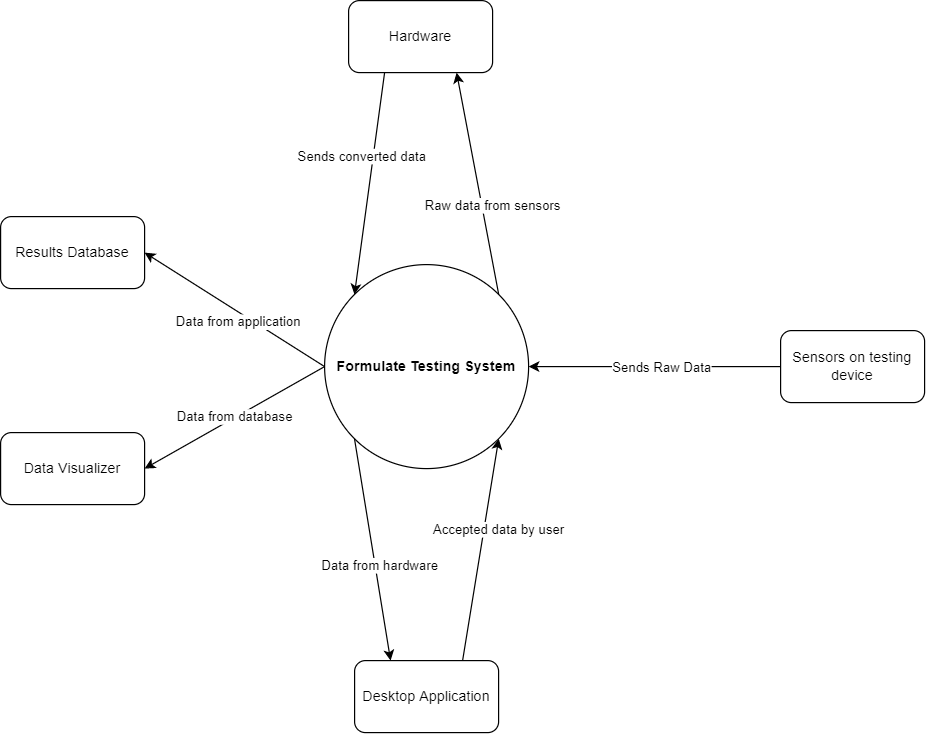
\includegraphics[width=0.9\textwidth]{sys_context_diagram}
\caption{System Context Diagram}
\label{Fig_SystemContext} 
\end{center}
\end{figure}

\subsection{State Transition Diagram}

\subsection{Monitored and Controlled Variables}
  \begin{tabular}{| p{0.23\textwidth} | p{0.10\textwidth}| p{0.10\textwidth}| p{0.46\textwidth}|}
    \hline
    \rowcolor[gray]{0.9}
    Monitored Variable & Type & Units & Description\\
    \hline
    m\_vibration & Analog& V& A signal monitoring the vibration resistance of the motor \\
    \hline
    m\_humidity & Analog & V & A signal monitoring the humidity of the motor’s environment \\
    \hline
    m\_temperature & Analog & V & A signal monitoring the temperature of the motor’s environment \\
    \hline
    m\_shock & Analog & V & A signal monitoring the shock resistance of the motor \\
    \hline
    m\_conv\_vibration & Digital & g  & Converted vibration values that are in useful units \\
    \hline
    m\_conv\_humidity & Digital & \% & Converted humidity values that are in useful units \\
    \hline
    m\_conv\_temperature & Digital & \textdegree C & Converted temperature values that are in useful units \\
    \hline
    m\_conv\_shock & Digital & g & Converted shock values that are in useful units \\
    \hline
    m\_data\_accepted & Digital & T/F & Determines if user has accepted the results and wants to send it to the database \\
    \hline
  \end{tabular}
\\Table 1.0: Monitored Variables\\ \\ \\
\begin{tabular}{| p{0.23\textwidth} | p{0.10\textwidth}| p{0.10\textwidth}| p{0.46\textwidth}|}
    \hline
    \rowcolor[gray]{0.9}
    Controlled Variable & Type & Units & Description\\
    \hline
    c\_green\_light& Digital& 1/0& Green LED light on testing device that indicates passed measurements \\
    \hline
    c\_red\_light& Digital & 1/0 & Red LED light on testing device that indicates failed measurements \\
    \hline
    c\_sent\_to\_database & Digital & T/F & Determines if results displayed on the application are sent to the database \\
    \hline
  \end{tabular}
  \\Table 2.0: Controlled Variables\\
  \begin{tabular}{| p{0.23\textwidth} | p{0.10\textwidth}| p{0.10\textwidth}| p{0.46\textwidth}|}
    \hline
    \rowcolor[gray]{0.9}
    Constant & Units & Value & Description\\
    \hline
    k\_temperature\_range& \textdegree C& 5-40& Acceptable ambient temperature values for a Formula Electric motor \\
    \hline
    k\_humidity\_range& \% & 5-85 & Acceptable relative humidity values for a Formula electric motor \\
    \hline
    k\_max\_shock & g & 100 & Maximum shock resistance for a Formula Electric motor \\
    \hline
    k\_max\_vibration & g & 20 & Maximum vibration resistance for a Formula Electric motor \\
    \hline
  \end{tabular}
  \\Table 3.0: Controlled Variables\\
\subsection{Functional Decomposition Diagram}
\begin{figure}[h!]
  \begin{center}
  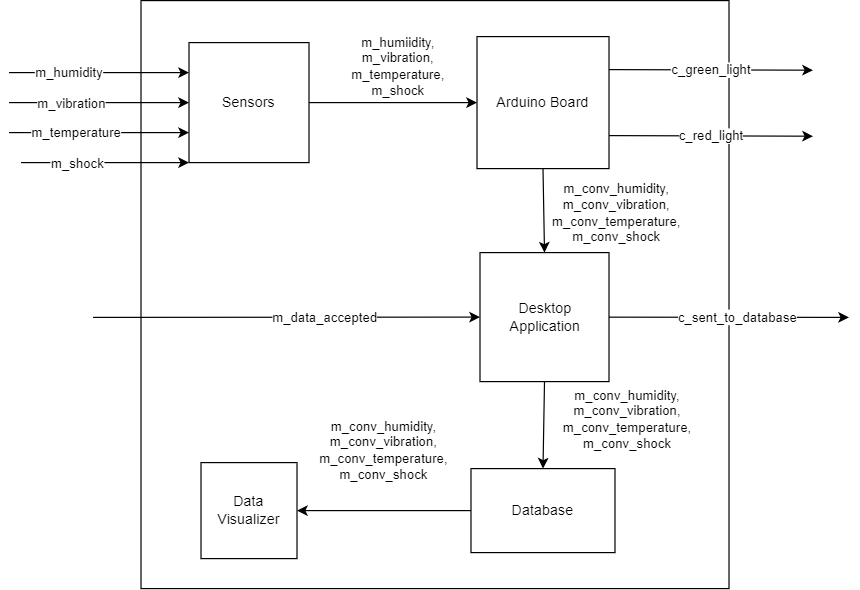
\includegraphics[width=0.9\textwidth]{functional_decomposition}
  \caption{Functional Decomposition Diagram}
  \label{Fig_FunctionalDecomposition} 
  \end{center}
  \end{figure}

\section{Requirements}

This section provides the functional requirements, the business tasks that the
software is expected to complete, and the nonfunctional requirements, the
qualities that the software is expected to exhibit.

\subsection{Functional Requirements}
Formulate consists of 3 main components, each with its own functional requirements. The hardware section addresses the sensors and physical device which interacts directly with the user, the desktop application is the means for the user to select modes and submit data and the data analytics platform is for the user to view old test case data to check if KPIs are met.

\subsubsection{Priority 1} 

\begin{itemize}
  \item[FR \refstepcounter{reqnum}\thereqnum:] The base device should contain a rechargeable battery
  \begin{description} \item[Rationale:] The base device needs its own independent power source which will allow for it to be placed in areas without a power socket. \end{description}
  
  
  \item[FR \refstepcounter{reqnum}\thereqnum:] The base device should have a screen to display the current status to the user
  
  \item[FR \refstepcounter{reqnum}\thereqnum:] The base device should easily mount to the Formula SAE car
  
  \item[FR \refstepcounter{reqnum}\thereqnum:] The base device should connect to a PC wirelessly and wired to transmit data
  
  \item[FR \refstepcounter{reqnum}\thereqnum:] The base device should alert the user if any tests exceed the operating condition of the car
  \begin{description} \item[Rationale] If at any point during the test it exceed operating conditions, the base devices should make it obvious to the user  \end{description}

  \item[FR \refstepcounter{reqnum}\thereqnum:] The base device should have 5 connection ports to add module sensors to it
  \begin{description} \item[Rationale] Each connection port will make the device more modular and allow for users to add more sensors in the future for other tests.  \end{description}
  
  \item[FR \refstepcounter{reqnum}\thereqnum:] The modular sensors should have a snap on mounting mechanism to connect to the base
  \begin{description} \item[Rationale] Modular sensors need to have a rigid connection with the base board with minimal movement to get the most accurate values from the sensor  \end{description}
  
  \item[FR \refstepcounter{reqnum}\thereqnum:] The base device should have a start button which activates the telemetry between the PC and device and starts reading values
  
  \item[FR \refstepcounter{reqnum}\thereqnum:] The base device should have a stop button which stops the telemetry between the PC and device and stops reading values
  
  \end{itemize}


\subsubsection{Priority 2}
\begin{itemize}
  \item[FR \refstepcounter{reqnum}\thereqnum:] The application should show live raw data from the sensors
  
  
  
  \item[FR \refstepcounter{reqnum}\thereqnum:] The application should allow users to preview the data after a test
  
  \item[FR \refstepcounter{reqnum}\thereqnum:] The application should allow the user to send the data to the database
  
  \item[FR \refstepcounter{reqnum}\thereqnum:] The application should allow the user to trim the data before sending it to the database
  
  \item[FR \refstepcounter{reqnum}\thereqnum:] The application should allow the user to configure the base device's settings
  \begin{description} \item[Rationale:] The base device will need to have the wifi setting configured which will be done in the application \end{description}
  
  \end{itemize}

\subsubsection{Priority 3}
\begin{itemize}
  \item[FR \refstepcounter{reqnum}\thereqnum:] The website should only allow users who have access to view the data
  
  \item[FR \refstepcounter{reqnum}\thereqnum:] The website should have the option to filter out the data by test conducted
  
  \item[FR \refstepcounter{reqnum}\thereqnum:] The website should show whether the tests passed according to threshold values
  
  \item[FR \refstepcounter{reqnum}\thereqnum:] The application should allow the user to trim the data before sending it to the database
  
  \item[FR \refstepcounter{reqnum}\thereqnum:] Any data pushed to the database should not be editable by the user
  
  \end{itemize}




\subsection{Nonfunctional Requirements}

\noindent \begin{itemize}

\item[NFR\refstepcounter{nfrnum}\thenfrnum:]
  \textbf{Maintainability} 

\item[NFR\refstepcounter{nfrnum}\thenfrnum:]
  \textbf{Portability} 


\end{itemize}


\subsection{Likely Changes}    

\noindent \begin{itemize}

\item[LC\refstepcounter{lcnum}\thelcnum\label{LC_meaningfulLabel}:] Starting and stopping the device to get data using hardware
\begin{description} \item[Rationale:] When the device is connected to the computer we can remote start and stop it using software \end{description}

\item[LC\refstepcounter{lcnum}\thelcnum\label{LC_meaningfulLabel}:] The base data we are collecting (Vibration, Shock, Temperature, Humidity)
\begin{description} \item[Rationale:] Since the device is set to be modular we might change those initial values we are testing with other ones \end{description}


\end{itemize}

\subsection{Unlikely Changes}    

\noindent \begin{itemize}

\item[ULC\refstepcounter{ulcnum}\theulcnum:] The sensors will remain modular to adapt to different tests that need to be conducted
\begin{description} \item[Rationale:] The product should be expandable in the future to be able to test different values \end{description}

\end{itemize}

\section{Development Plan}



\newpage

\bibliographystyle {plainnat}
\bibliography {../../refs/References}

\newpage

\noindent \plt{The following is not part of the template, just some things to consider
  when filing in the template.}

\noindent \plt{Grammar, flow and \LaTeX advice:
\begin{itemize}
\item For Mac users \texttt{*.DS\_Store} should be in \texttt{.gitignore}
\item \LaTeX{} and formatting rules
\begin{itemize}
\item Variables are italic, everything else not, includes subscripts (link to
  document)
\begin{itemize}
\item \href{https://physics.nist.gov/cuu/pdf/typefaces.pdf}{Conventions}
\item Watch out for implied multiplication
\end{itemize}
\item Use BibTeX
\item Use cross-referencing
\end{itemize}
\item Grammar and writing rules
\begin{itemize}
\item Acronyms expanded on first usage (not just in table of acronyms)
\item ``In order to'' should be ``to''
\end{itemize}
\end{itemize}}

\noindent \plt{Advice on using the template:
\begin{itemize}
\item Difference between physical and software constraints
\item Properties of a correct solution means \emph{additional} properties, not
  a restating of the requirements (may be ``not applicable'' for your problem).
  If you have a table of output constraints, then these are properties of a
  correct solution.
\item Assumptions have to be invoked somewhere
\item ``Referenced by'' implies that there is an explicit reference
\item Think of traceability matrix, list of assumption invocations and list of
  reference by fields as automatically generatable
\item If you say the format of the output (plot, table etc), then your
  requirement could be more abstract
\end{itemize}
}

\end{document}